\section{Методы детекции}

В силу сложности задачи детекции машинно-сгенерированного текста~--- как бинарной детекции, так и выделения фрагментов~--- модель для решения этой задачи должна хорошо понимать естественный язык. В частности, модели должны уметь искать не только явные отличия в стилистике текстов, но и скрытые признаки искусственной природы текста. Например, модели генерации с детерминированным способом семплирования следующего слова в тексте довольно легко могут детектироваться в силу того, что можно подсчитать внутренние характеристики текста, такие как перплексия или логарифмическая вероятность и в случае совпадения смоделированного текста и поданного на детекцию текста, можно сделать вывод, что данный текст является машинно-сгенерированным. Однако, на данный момент, модели с детерминированной стратегией генерации почти не используются, поэтому чаще используют модели-нейронные сети на основе трансформерной~\cite{Vaswani2017AttentionIA} архитектуры. Слой внимания в трансформерах позволяет учитывать контекст, что особенно важно для детекции фрагментов внутри документа, ведь необходимо сравниваться с другими фрагментами документами.

Кроме того, неоспоримым плюсом построения модели на основе трансформеров является наличие большого числа уже предобученных моделей, которые можно найти в открытом доступе. Взяв  предобученную модель,которая уже обладает хорошим уровнем понимания естественного языка, можно уже дообучить ее под конкретную задачу~--- например, на задачу бинарной классификации текста. Помимо этого, с точки зрения сложности реализации и затрат вычислительных ресурсов, дообучение существующей модели под конкретную задачу гораздо выгоднее, чем обучение модели с нуля. 
В данной главе векторные представления текстовых единиц, таких как предложения и параграфы, получаются с помощью токенизации с помощью предобученного энкодера на основе модели BERT~\cite{bert}. BERT является одной из классических трансформерных моделей и  на данный момент использование различных предобученных моделей на его основе является стандартным подходом токенизации текстов. 


\subsection{Модель для бинарной детекции}
\label{binary}

Так как в данной подзадаче требуется определить автора всего документа, то для классификации предлагается векторные представления документов передавать в линейный слой и после получения логитов для каждого токена в документе, выбирать автора документа по токену $[$CLS$]$, который является специальным токеном для всех BERT-энкодеров, предназначенным для классификации.



\subsection{Модель для детекции фрагментов}
\label{fragments}

Если известно по каким фрагментам проходит граница, то задача сводится к задаче бинарной классификации фрагментов и агрегированию полученных метрик бинарной классификации. Однако, в данном случае если каждый фрагмент оценивается отдельно, то никак не учитывается контекст фрагмента, например предыдущий параграф или предложение, а это может быть полезно при детекции автора текущего фрагмента. Для того чтобы учитывать контекст, предлагается использовать модель с марковским случайным полем (от англ. Conditional Random Fields), а точнее с марковской линейной цепочкой.
Пусть для документа $\mathbf{D} \in \mathbb{D}$ известны его параграфы $\mathcal{P} = (p_1, \dots, p_n)$ и $\mathbf{x} = (\mathbf{x}_1, \dots, \mathbf{x}_n)$~---векторные представления соотвествующих параграфов. Необходимо построить вероятностную модель $$p(y_1, \dots, y_n | \mathbf{x}_1, \dots, \mathbf{x}_n) = p(\mathbf{y} | \mathbf{x})$$
где $\mathbf{x}_i$~--- векторное представление параграфа $p_i$, $y_i$~--- автор параграфа $p_i$.

Ключевой идеей моделей с марковскими случайными полями  является введение вектора признаков
$$\Phi(\mathbf{x}, \mathbf{y}) \in \mathbb{R}^d$$
Функция $\Phi$ отображает последовательность векторных представлений и последовательность тегов-авторов в некоторый вектор признаков в пространстве $\mathbb{R}^d$, при этом каким-то образом учитывая зависимости между $\mathbf{x}_i$ и  $y_i$ и между соседними тегами $y_i$ и $y_{i-1}$.
Тогда вероятность получить последовательность тегов для данного документа выражается как:
\begin{equation}
\label{probability}
    p(\mathbf{y} | \mathbf{x}) = \frac{\exp\Phi(\mathbf{x},\mathbf{y})}{\sum\limits_{\mathbf{y}' \in \mathcal{Y}^n}\exp(\Phi(\mathbf{x},\mathbf{y}'))},
\end{equation}
где $\mathcal{Y}^n$ – множество всех возможных последовательностей тегов-авторов длины $n$  - в случае бинарной задачи это, по сути, все последовательности из 0 и 1 длины $n$.
В  общем случае, можно записать следующую зависимость:
$$ p(\mathbf{y} | \mathbf{x}) \propto  \prod_{i=1}^n \exp(\phi_i(y_{i-n},\dots, y_i, \mathbf{x}, i),$$
где функции $\phi_i$ отвечают за извлечение полезных для определения авторства признаков и определены как 
$$\Phi = \sum_{i=1}^n \log \phi_i(y_{i-k},\dots, y_i, \mathbf{x}, i),$$
где $k$ является размером контекстного окна, которое влияет на текущее предсказание. 
Для  задачи детекции достаточно будет взять $k = 1$ и зависеть только от предыдущего параграфа.

Перейдем к рассмотрению вида непосредственно функций $\phi_i$. Предлагается использовать две функции, первая из которых соотносит вероятность сопоставления тега $y_i$ с векторным представлением $\mathbf{x}_i$. Данная функция называется ``выхлопом'' (от англ. emissions), так как эти значения будут передаваться слою с марковской линейной цепочкой от какой-то другой модели, например из энкодера, LSTM-слоя или полносвязного слоя. На рис. \ref{BERT_CRF} показана схема использования CRF-слоя вместе с энкодером на основе BERT. Вторая функция устанавливает вероятности  появления тегов $y_i$ и $y_{i-1}$ в качестве соседей. Данная функция обычной называется ``переходом'' (от англ. transitions). Таким образом, функция $\Phi$ определена как:
\begin{equation}
\label{phi}
\Phi(\mathbf{x}, \mathbf{y}) = \log \phi_{\texttt{EMIT}} (y_1 \rightarrow x_1) + \sum\limits_{i=2}^{n} (\log \phi_{\texttt{EMIT}} (y_i \rightarrow x_i) + \log \phi_{\texttt{TRANS}} (y_{i - 1} \rightarrow y_i)).
\end{equation}
\begin{figure}[t!] %!t
\centering
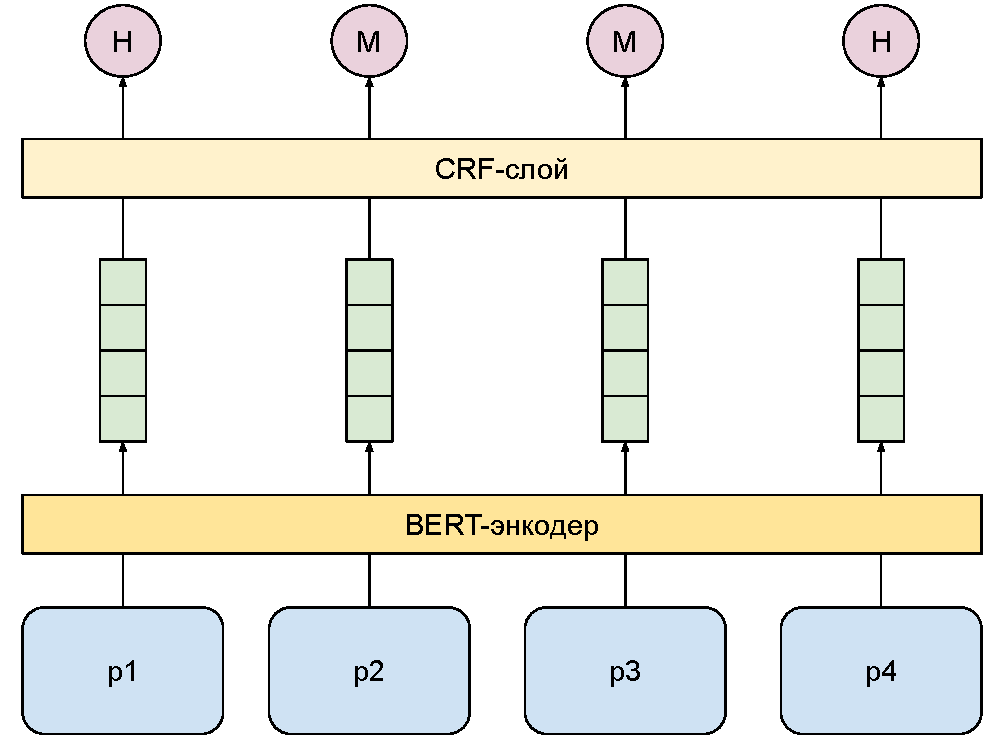
\includegraphics[width=0.7\linewidth]{images/BERT_CRF.pdf}
\caption{Схема модели с марковской линейной цепочкой. После применения модели каждому параграфу документа присваивается тег ``H'' для параграфа, написанного человеком и тег ``M'' для параграфа, сгенерированного большой языковой моделью}
\label{BERT_CRF}
\end{figure}


Задача обучения ставится как задача минимизации негативного логарифмического правдоподобия (Negative Log-Likelihood):
\begin{multline}
\label{loss}
    \mathcal{L}(\mathbf{Y}, \mathbf{X}) = - \log(p(\mathbf{Y} | \mathbf{X})) = - \sum\limits_{i = 1}^{n} \log(p(\mathbf{y}^i | \mathbf{x}^i)) = 
\cr = \sum\limits_{i = 1}^{n}  \Big(\log \Big [\sum\limits_{\mathbf{y}' \in \mathcal{Y}^n}\exp(\Phi(\mathbf{x}^i,\mathbf{y}'))\Big] - \Phi(\mathbf{x}^i, \mathbf{y}^i)\Big),
\end{multline}
где $\mathbf{X}, \mathbf{Y}$ - обучающая выборка. $\mathbf{y}^i \in \mathbf{Y}, \mathbf{x}^i \in \mathbf{X}$
Основная вычислительная сложность лежит в вычислении первого выражения в слагаемых в выражении \ref{loss}, так как необходимо вычислить переходы для всех возможных последовательностей тегов, что в случае очень длинных последовательностей или последовательностей в большим количеством возможных тегов невозможно. Однако, используя динамическое программирование и алгоритм Витерби~\cite{Viterbi} можно достаточно эффективно вычислить знаменатель.

Обозначим матрицу переходов, состоящую из значений функции $\phi_{\texttt{TRANS}}$, как $T$:
\begin{equation}
\label{matrix}
T[i][j] := \phi_{\texttt{TRANS}}(y_i \rightarrow y_j).
\end{equation}
Введем функцию $\pi[i][j]$, которая будет вычисляться как логарифм всех скоров последовательностей от 1ого параграфа и до $i + 1$-ого параграфа, так, что тег последнего параграфа будет равен $j$:
\begin{equation}
\label{pi}
\pi[i][j] = \log\sum\limits_{\mathbf{y} \in \mathcal{Y}^{i+1}} \exp(\Phi(\mathbf{x},\mathbf{y})).
\end{equation}

База рекурсии: 
\begin{equation}
\label{recursion_base}
\overrightarrow{\pi[0]} = \overrightarrow{T[0]} + \overrightarrow{\phi_{\texttt{EMIT}}(y_0 \rightarrow x_0)}.
\end{equation}
Докажем, что мы можем определять $\pi[i][j]$ рекурсивно.
\begin{proposition}
$\pi[i][j]$ выражается через $\pi[i - 1][j]$.
\end{proposition}

\begin{proof}
Докажем, что рекурсия корректна. По определению $\Phi(\mathbf{x},\mathbf{y'})$
\begin{multline}
\label{p_i_1}
    \pi[i-1][j] = \log \sum\limits_{\substack{y' \in \mathcal{Y}^{i} \\ y'[{-1}] = \mathcal{Y}[j]}} \exp\Big[\sum\limits_{k = 1}^{i - 1} \Big(\log \phi_{\texttt{EMIT}} (y'_k \rightarrow x_k)
    \cr + \log \phi_{\texttt{TRANS}} (y'_{k - 1} \rightarrow y'_k)\Big)\Big]
\end{multline}
\begin{multline}
\label{p_i}
\pi[i][j] = \log \sum\limits_{\substack{y' \in \mathcal{Y}^{i + 1} \\ y'[{-1}] = \mathcal{Y}[j]}} \exp\Big[\sum\limits_{k = 1}^{i } \Big(\log \phi_{\texttt{EMIT}} (y'_k \rightarrow x_k) 
    \cr + \log \phi_{\texttt{TRANS}} (y'_{k - 1} \rightarrow y'_k)\Big)\Big]
\end{multline}
Распишем правую часть равенства \ref{p_i}, сделав ``шаг назад'' и перебрав все возможные теги, которые могут стоять на $i - 1$ позиции:
\begin{multline*}
\pi[i][j] = \log \sum\limits_{t = 1}^{|\mathcal{Y}|} \sum\limits_{\substack{y' \in \mathcal{Y}^{i} \\ y'[{-1}] = \mathcal{Y}[t]}} \exp\Big[\log\phi_{\texttt{EMIT}} (y_i \rightarrow x_i) + \log\phi_{\texttt{TRANS}} (\mathcal{Y}[t] \rightarrow \mathcal{Y}[j]) +
\cr + \sum\limits_{k = 1}^{i - 1} \Big(\log \phi_{\texttt{EMIT}} (y'_{k} \rightarrow x_k) + \log \phi_{\texttt{TRANS}} (y'_{k - 1} \rightarrow y'_k)\Big)\Big] =
\cr = \log \sum\limits_{t = 1}^{|\mathcal{Y}|} \sum\limits_{\substack{y' \in \mathcal{Y}^{i} \\ y'[{-1}] = \mathcal{Y}[t]}} \exp\Big[\sum\limits_{k = 1}^{i - 1} \Big(\log \phi_{\texttt{EMIT}} (y'_{k} \rightarrow x_k) + \log \phi_{\texttt{TRANS}} (y'_{k - 1} \rightarrow y'_k)\Big)\Big] \cdot
\cr \cdot \phi_{\texttt{EMIT}} (y_i \rightarrow x_i) \cdot \phi_{\texttt{TRANS}} (\mathcal{Y}[t] \rightarrow \mathcal{Y}[j])
\end{multline*}
С учетом равенства \ref{p_i_1}
\begin{multline*}
\pi[i][j] = \log \sum\limits_{t = 1}^{|\mathcal{Y}|} \Big[\pi[i - 1][j]\cdot \phi_{\texttt{EMIT}} (y_i \rightarrow x_i) \cdot \phi_{\texttt{TRANS}} (\mathcal{Y}[t] \rightarrow \mathcal{Y}[j])\Big] = 
\cr = \log \sum\limits_{t = 1}^{|\mathcal{Y}|} \exp \Big[\pi[i - 1][t]+ \log⁡ \phi_\texttt{EMIT}(y_i \rightarrow x_i)+\log⁡ \phi_\texttt{TRANS}(\mathcal{Y}[t] \rightarrow \mathcal{Y}[j])\Big] 
\end{multline*}
\end{proof}
Таким образом, умея быстро подсчитывать функцию $\pi[i]][j]$, мы можем и быстро считать функцию потерь~\ref{loss}.


Чтобы восстанавливать последовательность тегов для некоторого документа с помощью марковской цепочки, формально нужно найти такую последовательность тегов, которая является наиболее вероятной для данного документа $\mathbf{x}$:
\begin{multline*}
\arg\max\limits_{y \in \mathcal{Y}^{n}} p(\mathbf{y}'|\mathbf{x}) = \arg\max\limits_{y \in \mathcal{Y}^{n}} \frac{\exp(\mathbf{\Phi}(\mathbf{x}, \mathbf{y}))}{\sum\limits_{\mathbf{y}' \in \mathcal{Y}^n} \exp(\mathbf{\Phi}(\mathbf{x}, \mathbf{y'})))} = \arg\max\limits_{y \in \mathcal{Y}^n} \mathbf{\Phi}(\mathbf{x}, \mathbf{y}) = 
\cr =\arg\max\limits_{y \in \mathcal{Y}^n} \sum\limits_{i = 2}^{n} (\log \phi_{\texttt{EMIT}} (y_i \rightarrow x_i) + \log \phi_{\texttt{TRANS}} (y_{i - 1} \rightarrow y_i))
\end{multline*}
Данные значения можно считать точно также с помощью динамического программирования, и функции $\pi[i][j]$, которая хранит максимальное суммарное значение скоров для всех последовательностей длины $i + 1$, последний тег которых соотвествует $j$. Сохраняя на каждом шаге индексы, на которых достигается максимум, мы можем восстановить последовательность тегов.


\subsection{Модель для детекции единственной смены авторов}

Введем функцию-детектор с параметром скользящего окна $\ell$, которая для токена в документе $d \in \mathbf{D}$ оценивает его вероятность быть токеном, в котором сменяются авторы:

\begin{equation}
    \mathbf \phi_{\ell} : \mathbb{D} \times \mathbb{N}_0 \quad \phi_{\ell}(\mathbf{D}, i) = \mathbb{P}(t_{i} = 1 | t_{i - \ell}, t_{i - \ell + 1}, ..., t_{i- 1})
\end{equation}
\begin{equation}
I_d = \arg \max_{0 \leq i \leq |d|} \phi_{\ell}(d, i)
\end{equation}
